\section{趋近的严格表述}
\label{sec:02-Calculus/02-Limits-and-Continuity/02}

日常语言里的``接近''太模糊了。如果说``当 \(x\) 靠近 2 时，\(f(x)\) 靠近 4''，这只能算一句直觉上的描述——因为没有任何办法去检验它到底对不对。

要让这句话变得严密，我们需要把它变成一场``确定误差范围的游戏''：

我不直接喊``\(f(x)\) 靠近 4''，而是向你下战帖：
\begin{itemize}
  \item \textbf{你来当挑剔的裁判}：你可以提出任意苛刻的误差要求，比如``我要 \(f(x)\) 与 4 的距离必须小于 0.01''；
  \item \textbf{我来当应战的选手}：我必须找到一个足够小的 \(x\) 范围（比如``只要 \(x\) 与 2 的距离控制在 0.005 以内''），保证在这个范围里的每一个 \(x\)，算出来的 \(f(x)\) 都能满足你的要求。
\end{itemize}

如果不管你把误差要求提得有多高（哪怕收紧到 0.00001 甚至任意小），我都总能找到一个对应的 \(x\) 范围来应对，那么我们才能底气十足地说：当 \(x\to 2\) 时，\(f(x)\) 的极限就是 4。

极限的严格定义，无非就是把这个游戏里的具体数字，换成两个代表``允许误差''和``控制范围''的数学符号。

还记得上一节最后的那个争论吗？——有人硬说 \(\lim_{x\to1} \frac{x^2-1}{x-1} = 1.999\)。在这个规则下，你只需要提出一个稍高一点的精度要求（例如``误差必须小于 0.0001''），他就再也给不出任何能满足要求的 \(x\) 范围，这个假说法就会被彻底驳倒。

\subsection{极限的严格定义（\(\varepsilon\)-\(\delta\) 语言）}

断言 \(\lim_{x\to a}f(x)=L\)，本质上就是应付这场``误差与范围''的逻辑博弈。

这场游戏的规则可以清晰地拆解为两步：
\begin{enumerate}
  \item \textbf{对方先出手（指定精度）}：对方报出一个任意小的正数 \(\varepsilon\)（读作 epsilon），代表他能接受的最大输出误差。只要设定了 \(\varepsilon\)，函数值 \(f(x)\) 就必须被限制在区间 \((L-\varepsilon, L+\varepsilon)\) 内。
  \item \textbf{你来作回应（控制范围）}：你需要找到一个正数 \(\delta\)（读作 delta）。只要输入 \(x\) 与 \(a\) 的距离控制在 \(\delta\) 之内（即落在区间 \((a-\delta, a+\delta)\) 内，但除去 \(a\) 本身），函数值 \(f(x)\) 就绝对不会超出对方设定的误差范围。
\end{enumerate}

只要无论对方提出多么苛刻的 \(\varepsilon\)，你都能找到对应的 \(\delta\) 来应战，极限 \(\lim_{x\to a}f(x)=L\) 就正式成立。相反，如果对方找到了某个 \(\varepsilon\)，让你无论怎么缩小 \(\delta\) 都会产生越界的``坏点''，你就输了，极限也就不存在。

用数学语言将这场游戏规范地写出来，就是微积分中最核心的定义：

\begin{definition}
\(\lim_{x\to a}f(x)=L\) 意指：对于任意给定的 \(\varepsilon>0\)，都存在一个 \(\delta>0\)，使得当 \(0<|x-a|<\delta\) 时，必有
\[
|f(x)-L|<\varepsilon.
\]
\end{definition}

注意不等式最左侧的 \(0<|x-a|\)：它唯独排除了 \(x=a\) 这个点。这意味着，无论 \(f(a)\) 有没有定义、或者定义成什么值，都完全不影响极限是否存在。上一节讨论的``空心点''情况，在这里得到了严密的数学许可。

\begin{center}
\begin{tikzpicture}[x=1.35cm,y=1.2cm,font=\small,>=stealth]
  \fill[red!12] (-0.1,1.55) rectangle (3.5,2.45);
  \fill[blue!14] (1.55,-0.1) rectangle (2.45,3.3);
  \draw[->] (-0.2,0) -- (3.7,0) node[right] {\(x\)};
  \draw[->] (0,-0.2) -- (0,3.55) node[above] {\(y\)};
  \draw[blue!70!black,thick] plot[domain=0.2:3.3,samples=60] (\x,{0.8+0.42*\x+0.09*\x*\x});
  \draw[black!55,dashed] (-0.1,2) -- (3.5,2);
  \draw[black!55,dashed] (2,-0.1) -- (2,3.3);
  \node[left,red!60!black,font=\footnotesize] at (-0.15,2.45) {\(L+\varepsilon\)};
  \node[left,red!60!black,font=\footnotesize] at (-0.15,1.55) {\(L-\varepsilon\)};
  \node[left] at (-0.15,2) {\(L\)};
  \node[below] at (2,-0.12) {\(a\)};
  \node[below,blue!55!black,font=\footnotesize] at (1.55,-0.5) {\(a-\delta\)};
  \node[below,blue!55!black,font=\footnotesize] at (2.45,-0.5) {\(a+\delta\)};
  \node[right,red!60!black,font=\footnotesize] at (3.55,2.0) {对方先画出水平误差带};
  \node[above,blue!55!black,font=\footnotesize] at (2.0,3.35) {你再给出垂直控制区间};
\end{tikzpicture}

\emph{水平误差带的高度由对方指定，垂直控制区间的宽度由你来回应。判定标准很简单：只要在这个垂直区间内的函数图像，完全被包含在水平误差带内部即可。误差带压得越扁，你通常就需要把控制区间收得越窄。}
\end{center}

结合几何图形，有两点逻辑顺序极其关键：
\begin{enumerate}
  \item \textbf{顺序不能颠倒}：水平带必须先画——你的 \(\delta\) 是根据对方给的 \(\varepsilon\) 来挑选的，先有要求，后有回应。
  \item \textbf{一选定即全覆盖}：你的 \(\delta\) 一旦选定，就必须对这个区间内的\textbf{所有} \(x\) 统统生效，绝不能针对不同的 \(x\) 临时修改 \(\delta\)。
\end{enumerate}

不妨思考一下：如果把公式里``\(\forall\varepsilon>0,\;\exists\delta>0\)''的顺序颠倒过来，变成``\(\exists\delta>0,\;\forall\varepsilon>0\)'',会发生什么？

这意味着``先选定一个固定的范围 \(\delta\)，要求它能满足\textbf{任意}小的误差 \(\varepsilon\)''。这说明在这个范围里，函数值与 \(L\) 的距离必须比任何正数都小——也就是说，函数在这个区间内只能是常数。量词顺序一旦变更，极限的本质含义就彻底改变了。

\subsection{构造证明的两步法：先定范围，再配误差}

具体怎么凑出 \(\delta\) 的技巧其实并不复杂，它的核心骨架只有两步。弄懂了这个逻辑，整章的论证就通透了。

对于最简单的线性函数，几乎不需要动脑筋。比如证明 \(\lim_{x\to2}(3x+1)=7\)：
因为误差为 \(|(3x+1)-7|=3|x-2|\)，我们要让误差小于 \(\varepsilon\)，只需直接令 \(|x-2|<\varepsilon/3\)。所以取 \(\delta=\varepsilon/3\) 即可。由于输入偏差与输出误差之间只是固定的常数倍关系，把常数直接除过去就解决了。

真正麻烦的是\textbf{系数随 \(x\) 变化}的情况。比如证明 \(\lim_{x\to2}x^2=4\)：
此时误差为 \(|x^2-4|=|x-2|\cdot|x+2|\)。前面的 \(|x-2|\) 是我们可以用 \(\delta\) 直接控制的，但后面的 \(|x+2|\) 却会随着 \(x\) 的变动而变动。

解决办法是\textbf{分两步走}：
\begin{enumerate}
  \item \textbf{第一步（先给 \(x\) 划定一个初步范围）}：先随便给 \(x\) 一个宽松的限制，比如要求 \(|x-2|<1\)。这就把 \(x\) 限制在了区间 \((1,3)\) 内。在这个范围内，\(|x+2|\) 最大也不会超过 \(5\)（即 \(|x+2|<5\)）。这样，我们就把浮动的变量成功``封顶''成了一个具体的数字 \(5\)。
  \item \textbf{第二步（根据上界分配误差）}：有了上界 \(5\)，我们只需要再额外要求 \(|x-2|<\varepsilon/5\)，总误差 \(|x-2|\cdot|x+2|\) 就会被稳稳限制在 \(\varepsilon\) 以内。
\end{enumerate}

由于这两个限制条件必须\textbf{同时满足}，所以最终的 \(\delta\) 必须取两者的最小值：
\[
\delta=\min\{1,\;\varepsilon/5\}.
\]
这里的 \(\min\) 不是在摆弄形式，而是确保不管 \(\varepsilon\) 给得多大，\(x\) 都绝不会超出第一步预设的安全性范围。

这里还有一个初学者最容易混淆的\textbf{书写方向问题}：在草稿纸上算 \(\delta\) 时，我们是从目标误差 \(|f(x)-L|<\varepsilon\) \textbf{倒着推}输入范围 \(|x-a|\) 的；但在写正式证明时，必须\textbf{正着写}——先直接给出 \(\delta\)，再从 \(0<|x-a|<\delta\) 逐步正向推出``误差符合要求''。这就像在草稿纸上解谜可以倒推，但给别人演示逻辑时必须从起点正向推导一样。

此外，\(\delta\) 并不是唯一的，只要能解决问题，不一定要找``最优解''。比如取 \(\delta=\min\{0.5,\;\varepsilon/6\}\) 也完全合格。定义要求的只是``存在一个可行方案''，而不是``最优方案''。

\subsection{否定极限：寻找一个致命的 \texorpdfstring{\(\varepsilon_0\)}{epsilon0}}

如果要证明一个极限\textbf{不存在}（或者否定一个错误的极限），角色就会对调：此时你需要主动出击，找到一个具体的致命误差 \(\varepsilon_0\)。无论对方把 \(\delta\) 窗口收得有多窄，你都能在这个窗口内挑出一个越界的``坏点''。

用逻辑语言把``存在极限''的反面写出来，就是：
\[
\exists\varepsilon_0>0,\;\forall\delta>0,\;
\exists x:\;0<|x-a|<\delta\;\text{且}\;|f(x)-L|\ge\varepsilon_0.
\]

回想上一节符号函数 \(\operatorname{sgn}(x)\) 的例子：在 \(x=0\) 的左边函数值恒为 \(-1\)，右边恒为 \(1\)。如果你宣称极限是某个数 \(L\)，因为 \(1\) 到 \(-1\) 的总距离是 \(2\)，无论你把 \(L\) 定在什么高度，它到 \(1\) 或到 \(-1\) 的距离中，\textbf{至少有一边不小于 1}。

这就给了我们绝杀的机会：直接报出 \(\varepsilon_0=1\)。接下来，不管对方给出的 \(\delta\) 窗口有多小，只要 \(L\) 偏向左边，你就去右半窗口挑点（此时函数值为 \(1\)，误差大于等于 \(1\)）；只要 \(L\) 偏向右边，你就去左半窗口挑点。无论窗口缩得有多微小，坏点永远在那里等着他。因此没有任何候选值 \(L\) 能通过检验，极限根本不存在。

这个套路适用于所有出现``断层''或``剧烈摆动''的函数：只要函数在目标点附近呈现出两群互不相容的取值，两群取值间距的一半，就是那个能把假极限当场卡死的 \(\varepsilon_0\)。

对于上一节那个硬说 \(\lim_{x\to1}\frac{x^2-1}{x-1}=1.999\) 的杠精，你现在只需要亮出 \(\varepsilon_0=0.0005\)。因为只要 \(x\) 足够靠近 \(1\)，真正的函数值其实无限接近于 \(2\)，与 \(1.999\) 的距离必然会保持在 \(0.0009\) 左右（大于 \(0.0005\)）。他给不出任何能同时满足要求的 \(x\) 范围，争论立刻结束。

\subsection{\texorpdfstring{\(\delta\)}{delta} 能看清谁，决定了你拿到的是哪种控制力度}

现在，把注意力从``怎么凑 \(\delta\)''转移到一个更本质的问题上：\(\delta\) 允许和哪些量挂钩？

\(\delta\) 必须根据 \(\varepsilon\) 来挑选，这是逻辑的核心。同时，它也可以依赖具体的函数 \(f\) 以及目标点 \(a\)——因为在函数的不同位置，同样的精度要求可能需要宽窄悬殊的控制范围。但是，\textbf{\(\delta\) 绝不能依赖具体的 \(x\)}，因为 \(\delta\) 必须在挑选 \(x\) 之前就确定下来。

允许 \(\delta\) 依赖于点 \(a\)，看似合情合理，但在某些情况下会带来意想不到的麻烦。

看函数 \(f(x)=1/x\) 在区间 \((0,1)\) 上的表现：固定精度要求 \(\varepsilon=0.5\)。
在 \(a=0.6\) 附近，函数曲线比较平缓，一个不算窄的 \(\delta\) 就能满足要求；但如果挪到靠近原点的 \(a=0.2\)，曲线陡峭得多，为了把高度差控制在 \(0.5\) 以内，横向的 \(\delta\) 窗口必须大幅收紧；如果再挪到 \(a=0.02\)，窗口更是得缩窄几个数量级。

\begin{center}
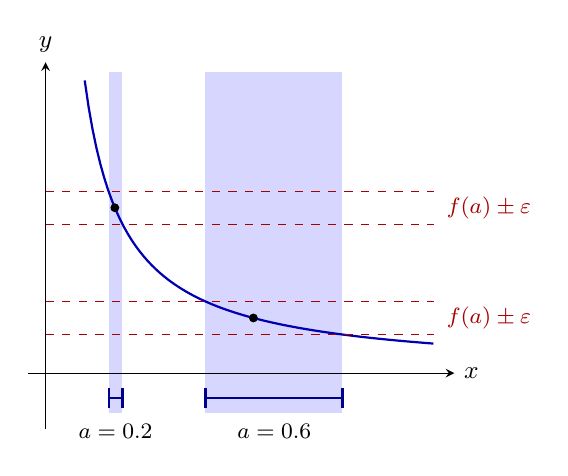
\begin{tikzpicture}[x=4.4cm,y=0.42cm,font=\small,>=stealth]
  \fill[blue!16] (0.182,-1.2) rectangle (0.222,9.1);
  \fill[blue!16] (0.4615,-1.2) rectangle (0.857,9.1);
  \draw[->] (-0.05,0) -- (1.18,0) node[right] {\(x\)};
  \draw[->] (0,-1.7) -- (0,9.4) node[above] {\(y\)};
  \draw[blue!70!black,thick] plot[domain=0.113:1.12,samples=90] (\x,{1/\x});
  \draw[red!65!black,dashed] (0,4.5) -- (1.12,4.5);
  \draw[red!65!black,dashed] (0,5.5) -- (1.12,5.5);
  \draw[red!65!black,dashed] (0,1.167) -- (1.12,1.167);
  \draw[red!65!black,dashed] (0,2.167) -- (1.12,2.167);
  \fill[black] (0.2,5) circle (1.6pt);
  \fill[black] (0.6,1.667) circle (1.6pt);
  \draw[blue!55!black,thick] (0.182,-0.75) -- (0.222,-0.75)
    (0.182,-0.45) -- (0.182,-1.05) (0.222,-0.45) -- (0.222,-1.05);
  \draw[blue!55!black,thick] (0.4615,-0.75) -- (0.857,-0.75)
    (0.4615,-0.45) -- (0.4615,-1.05) (0.857,-0.45) -- (0.857,-1.05);
  \node[below,font=\footnotesize] at (0.202,-1.25) {\(a=0.2\)};
  \node[below,font=\footnotesize] at (0.66,-1.25) {\(a=0.6\)};
  \node[right,red!65!black,font=\footnotesize] at (1.13,5.0) {\(f(a)\pm\varepsilon\)};
  \node[right,red!65!black,font=\footnotesize] at (1.13,1.667) {\(f(a)\pm\varepsilon\)};
\end{tikzpicture}

\emph{两对虚线之间的垂直高度相同（对应同一个 \(\varepsilon\)）。但因为曲线在越靠近原点处越陡峭，要想把函数值限制在这个高度内，左边的垂直控制窗口必须比右边窄得多。普通的极限允许``因地制宜''，每个点都可以配一套自己的 \(\delta\)。}
\end{center}

这就引出了一点自然的思考：\textbf{能不能找到一个通用的 \(\delta\)，让它对整条定义域上的所有点同时生效？}

这就是所谓的\textbf{一致连续}。对于 \(1/x\) 在 \((0,1)\) 上，这是做不到的，因为越靠近 \(0\) 要求的窗口就越窄，需要的宽度会一路缩到零，找不到一个固定的正数能``包办全场''；但如果把区间限制在 \([0.1,1]\) 上，曲线最陡峭的地方被挡在了外面，就能找到一个通用的 \(\delta\) 了。

量词位置的微小移动，对应着完全不同的控制强度。这种``局部控制''与``全局统一控制''的逻辑对比，在高等数学中会反复上演。

\subsection{这套定义不负责什么}

必须明确一点：\(\varepsilon\)-\(\delta\) 定义是一套\textbf{严格的检验标准}，而不是\textbf{求解答案的计算工具}。它能帮你判定一个给定的候选值 \(L\) 合不合格，但它本身绝对不会告诉你 \(L\) 到底是怎么算出来的。

能够用定义证明 \(\lim_{x\to2}x^2=4\)，和能够熟练计算复杂的 \(\lim_{x\to0}\frac{\sin(x^2)}{1-\cos x}\)，完全是两种不同的能力。前者靠的是严密的逻辑推导，后者依靠的是下一节要学习的极限运算法则与化简技巧。

初学者读到这里，完全没必要要求自己立刻就能为任意复杂的函数构造 \(\delta\)。合理的目标是：能够看懂一份写好的证明，分清哪一步是在给变量封顶、哪一步是在推导误差，能独立写出简单线性函数的证明，并理解为什么 \(\min\) 必须出现，就完全足够了。

定义的真正价值，在于它为``趋近''、``稳定''、``误差可控''这些日常概念提供了一个公认的、不可动摇的裁决标准，让你在面对复杂的数学推导时，心中始终有一块坚实的底座。

至于日常做题时如何避开繁琐的定义，高效地拆分、合并与计算极限，就是下一节要探讨的内容了。
